%%%%%%%%%%%%%%%%%%%%%%%%%%%%%%%%%%%%%%%%%%%%%%%%%%%
%%%%%%%% Präambel
%%%%%%%%%%%%%%%%%%%%%%%%%%%%%%%%%%%%%%%%%%%%%%%%%%%
\documentclass[a4paper, bibliography=totocnumbered, listof=totocnumbered, oneside, 12pt, ngerman]{scrbook}
\usepackage{geometry}
\geometry{a4paper,left=35mm,right=35mm,top=12mm,bottom=20mm, includeheadfoot}
\setlength\headheight{8mm}

% color
\usepackage{xcolor}
\definecolor{blue}{RGB}{0,128,255}
\definecolor{green}{RGB}{0,128,0}
\definecolor{orange}{RGB}{255,128,0}
\definecolor{lila}{RGB}{128,0,255}
\definecolor{black}{RGB}{0,0,0}

% Absätze
\parindent=0cm

%%%%%%%%%%%%%%%%%%%%%%%%%%%%%%%%%%%%%%%%%%%%%%%%%%%
%%%%%%%% packages
%%%%%%%%%%%%%%%%%%%%%%%%%%%%%%%%%%%%%%%%%%%%%%%%%%%

% speech
\usepackage[utf8]{inputenc}
\usepackage[ngerman]{babel}

% font
\usepackage{lmodern}
\renewcommand\textbullet{\ensuremath{\bullet}}

% hyperlinks
\usepackage[hyphens]{url}
\usepackage[hidelinks]{hyperref}

% math
\usepackage{mathrsfs}

% Bibliothek
\usepackage{bibgerm}
\bibliographystyle{alpha}

% graphics
\usepackage{graphicx}
\DeclareGraphicsExtensions{.pdf,.jpeg,.png,.jpg}

% pseudocode
\usepackage{algpseudocode}

% theorem
\usepackage{amsthm}
\newtheorem{theorem}{Theorem}
\newtheorem{definition}{Definition}

% Codebeispiel
\usepackage{scrhack}
\usepackage{listings}
\renewcommand{\lstlistlistingname}{Quellcodeverzeichnis}
\renewcommand{\lstlistingname}{Codebeispiel}
\lstset{
  backgroundcolor=\color{white},
  basicstyle=\footnotesize,
  breakatwhitespace=false,
  breaklines=true,
  captionpos=b,
  commentstyle=\color{green},
  frame=single,
  keepspaces=true,
  keywordstyle=\color{blue},
  numbers=left,
  numbersep=5pt,
  showspaces=false,
  tabsize=2,
  xleftmargin=0.1\textwidth,
  xrightmargin=0.1\textwidth
}

%%%%%%%%%%%%%%%%%%%%%%%%%%%%%%%%%%%%%%%%%%%%%%%%%%%
%%%%%%%% Document
%%%%%%%%%%%%%%%%%%%%%%%%%%%%%%%%%%%%%%%%%%%%%%%%%%%
\begin{document}
\pagenumbering{roman}

\begin{titlepage}
\begin{centering}
\vspace*{\fill}

\vspace{3cm} 

\textbf { \LARGE
Hypertext-Systeme 1
\\(Lokale Systeme)
\\[1.2cm]
}

{\large
vorgelegt von:
}

\textbf { \Large
Kevin Haack\\[1cm]
}

{\large
Matrikelnummer: 7094226
\\[2mm]
}

{\large
Studiengang: Informatik (M.Sc.)\\[1cm]
}
    
{\large
Thema betreut von:
}

\textbf { \Large
Dr. Felix Winkelnkemper
\\[1cm]
}

{\large
Paderborn, \today
}
\vfill
\end{centering}
\end{titlepage}
\chapter*{Kurzzusammenfassung}

\begin{centering}
\textbf { \LARGE
Security of Symmetric Encryption against Mass Surveillance
\\[1.2cm]
}
\end{centering}

{\large
Zusammenfassung
}

{
Spätestens seit den Snowden Leaks ist öffentlich bekannt, dass Massen"-über"-wachung im Internet stattfindet. Codenamen wie PRISM werden in Zeitschriften ver"-öffentlicht (\cite{Guard}). Wir sehen, dass verschlüsselte Übertragungen unsere Daten nicht vor unbefugtem Zugriff schützen. Pseudozufallsgeneratoren die möglicherweise nicht ganz zufällig sind, wie zum Beispiel der NIST Dual EC DRBG, sorgen für potenziell unsichere VPN Verbindungen und Backdoors in eigentlich sicheren Übertragungen (\cite{dual}) könnten in nahezu jeder Anwendung vorkommen. Das original Paper von Mihir Bellare, Kenneth G. Paterson und Phillip Rogaway soll die erste Salve im Kampf gegen Massenüberwachung abgeben (\cite{praesi}) und fokussiert sich auf symmetrische Verschlüsselungsschemen und einen speziellen Angriffsvektor, den sogenannte Algorithm Substitution Attacks. Es soll eine Grundlage mit der Definition und Formalisierung schaffen für die Abwehr dieses Angriffs. Denn symmetrische Verschlüsselungen bilden das Rückkrad vieler alltäglicher Übertragungs"-techniken wie zum Beispiel IPsec oder TLS. Diese Arbeit soll zunächst einen Überblick über das Originalwerk geben, Inhalte zusammenfassen und verdeutlichen. Es wird dargestellt, wie Algorithm Substitution Attacks funktionieren könnten und welchen symmetrische Schemen dagegen gefeit sind.
}\vspace{12pt}

{\large
Stichworte
}

{
Algorithm Substitution Attacks, symmetrische Verschlüsselung, unique ciphertext scheme, key recovery
}

\tableofcontents
\cleardoublepage
\pagenumbering{arabic}

\chapter{Was ist Hypertext?}
\label{ch:Was ist Hypertext?}

\begin{section}{Was ist überhaupt Hypertext?}
\label{sec:big_brother}

Was ist überhaupt Hypertext? Nach Jakob Nielsen in dem Buch Multimedia and Hpertext: The Internet and Beyond aus dem Jahr 1995, ist:

\begin{quote}
\glqq The simplest way to define hypertext is to contrast it with traditional text like a book. All traditional text, whether in printed form or in computer files, is sequential, meaning that there is a single linear sequence defining the order in which the text is to be read. [...] Hypertext is nonsequential; there is no single order that determines the sequence in which the text is to be read.\grqq{ }\cite[S.1]{Nielsen1995}
\end{quote}

Jakob Nielsen beschreibt, genau wie Jeff Conklin in seinem Artikel Hypertext: An Introduction and Survey, Hypertext als Informationsquelle die dem Leser die Freiheit gibt die Informationen in beliebiger Reihenfolge abzurufen. Der Leser dürfe entscheiden, welche Links er nutze und in welcher Reihenfolge \cite[S.33]{Conklin1987} \cite[S.1]{Nielsen1995}.

\begin{quote}
\glqq Hypertext allows and even encourages the writer to make such references, and allows the readers to make their own decisions about which links to follow and in what order. In this sense, hypertext eases the restrictions on the thinker and writer. It does not force a strict decision about whether any given idea is either within the flow of a paper's stream of thought or outside of it.\grqq{ }\cite[S.33]{Conklin1987}
\end{quote}

Also könnte ein Hypertext wie auf Abbildung \ref{fig:nielsenLink} zu sehen, aus vielen einzelnen Informationen bestehen zwischen denen eine Verlinkung existiert. Durch diese Links kann der Leser entscheiden an welcher Stelle er weiter lesen möchte. Anstatt den Text in der festen Reihenfolge $A$, $B$, $C$, $...$ und dann $G$ zu lesen, gibt es für den Leser mehrere Möglichkeiten die Texte aufzurufen. Nach Text $A$ könne zum Beispiel sofort Text $D$ folgen und so weiter\cite[S.1]{Nielsen1995}.

\begin{figure}[H]
	\centering
	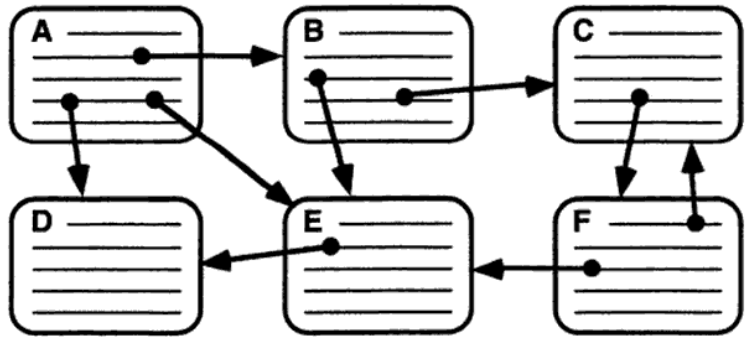
\includegraphics[width=0.8\textwidth]{image/nielsenLink}
	\caption{Vereinfachte Ansicht eines Hypertextes \cite[S.1]{Nielsen1995}}
	\label{fig:nielsenLink}
\end{figure}


Einen Hypertext kann oftmals als Graphen aus Knoten und Kanten dargestellt werden. Diese Darstellungsform kann vor dem Leser verborgen sein, muss es aber nicht \cite{Conklin1987}. Eine Information, ein Absatz, ein Text oder ein Dokument ist ein Knoten, die Größe spielt hierbei keine Rolle. Ein Knoten kann nun Links auf andere Knoten haben und diese sind dann die Kanten in dem Graphen \cite[S.19]{Conklin1987} \cite[S.2]{Nielsen1995}. Auch John B. Smith und Stephen F. Weiss schreiben in dem Artikel Hypertext vergleichbar über Hypertext als Netzwerk aus Informationen mit Links \cite{Smith1988}. Diese bezeichnen unter anderem auch Verlinkungen zwischen Medien wie Audio-, Grafik- oder Videodateien als Hypertext. In diesem Zusammenhang verwendet Theodor \glqq Ted\grqq{ }Holm Nelson auch den Begriff \glqq Hypermedia\grqq{ }\cite{Nelson1965}.

\begin{quote}
    \glqq [...] Hypertext is an approach to information management in which data is stored in a network of nodes connected by links. Nodes can contain text, graphics, audio, video, as well as source code or other forms of data.\grqq{ }\cite{Smith1988}
\end{quote}

Wie auf Abbildung \ref{fig:imText} zu sehen, müsse eine Link also nicht unbedingt von Wort zu Wort führen, sondern könne auch den Token $xxxx$ im Dokument $A$ mit dem ganzen Dokument $B$ verbinden \cite{Conklin1987}. 

\begin{figure}[H]
	\centering
	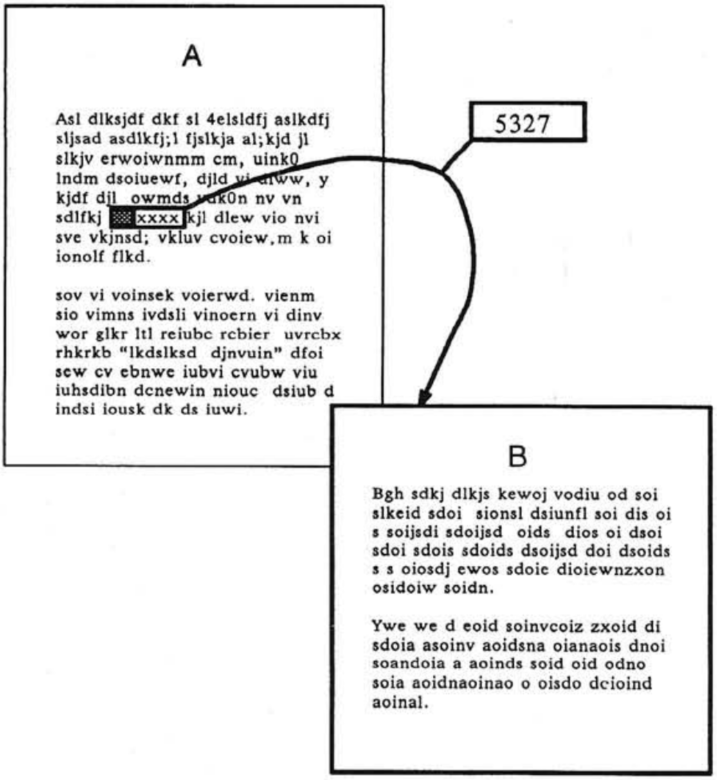
\includegraphics[width=0.8\textwidth]{image/imText}
	\caption{Ein Beispiel eines Links von in einem Text zu einem anderen Text \cite[S.34]{Conklin1987}}
	\label{fig:imText}
\end{figure}

\begin{quote}
    \glqq The same is true of footnotes in traditional printed texts, since readers have to determine upon reaching the footnote marker whether to continue reading the primary stream of text or to branch off to pursue the footnote. \grqq{ }\cite{Nielsen1995}
\end{quote}

Das gleiche könne auch auf einen traditionellen Text auf Papier zutreffen, Fußnoten referenzieren auf andere Texte und geben dem Leser die Möglichkeit an anderer Stelle weiterzulesen \cite{Nielsen1995}. Auch Ted Nelson schrieb in Literary Machines 1992:

\begin{quote}
\glqq By hypertext I simply mean non-sequential writing. A magazine layout, with sequential text and insert illustrations and boxes, is thus hypertext.\grqq{ }\cite{Nelson1992}
\end{quote} 

\end{section}

\begin{section}{Abgrenzung}
\label{sec:abgrenzung}

Doch für eine Antwort auf die Frage was ein Hypertext ist, gibt es sicherlich noch viele andere Antworten und Definitionen. Doch im Jahr 1945 veröffentlichte Vannevar Bush den Artikel \glqq As we may think\grqq{ }und formulierte darin die Grundidee zu Hypertext. Ich beschränke mich in dieser Arbeit auf lokale Hypertext-Systeme insbesondere der achtziger Jahre. Ich nehme in dieser Arbeit Bezug auf ausgewählte Hypertext-Systeme, deren Benutzung, Funktionen und technische Umsetzung. Ein besonderes Augenmerk legt diese Arbeit hierbei auf die Umsetzung der Links. Vernetzte und verteilte Hypertext-Systeme klammere ich in dieser Arbeit explizit aus.

\end{section}

\chapter{Grundlagen}
\label{ch:Grundlagen}

Dieses Kapitel soll eine Grundlage für jeden Leser schaffen. Es werden die grundlegenden Rahmenbedingungen beschrieben, erste Begriffe und Notationen eingeführt um das spätere Verständnis des Originalwerks zu erläutern. So wird auf den folgenden Seiten ein symmetrisches Verschlüsselungs"-schema $\Pi$ und dessen Subversion $\widetilde{\Pi}$ behandelt. Subversionen sind von $\mathscr{B}$ in das Schema eingeschleuste Komponenten, die ein Key Recovery ermöglichen sollen.

\begin{section}{Die ideale Welt}
\label{sec:ideale_welt}

Als Basis für alle Erläuterungen dient ein Model der idealen Welt (siehe Abbildung \ref{fig:ideale_welt}). In einer idealen Welt möchte Alice eine verschlüsselte Nachricht $M$ an Bob schicken. Alice und Bob sind normale Nutzer, die im Besitz eines symmetrischen Schlüssels $\mathcal{K}$ sind. Für diese Übertragung wird ein symmetrisches Verschlüsselungs"-schema $\Pi = (\mathcal{E}, \mathcal{D}, \mathcal{K})$ verwendet. Das Schema $\Pi$ besteht aus einer Funktion $\mathcal{E} = (\mathcal{K}, M)$, die mit dem symmetrischen Schlüssel $\mathcal{K}$ die Nachricht $M$ verschlüsseln und eine Funktion $\mathcal{D} = (\mathcal{K}, \mathcal{C})$, die mit dem symmetrischen Schlüssel $\mathcal{K}$ einen Chiffretext $\mathcal{C}$ entschlüsselt. So ergibt sich eine erste allgemeine Definition eines symmetrischen Verschlüsselungsschemas. Big Brother $\mathscr{B}$ versucht in diesem Fall passiv die Nachricht zu entschlüsseln oder den Schlüssel $\mathcal{K}$ zu reproduzieren. Diese Art von Darstellung von Abbildung \ref{fig:ideale_welt} werde ich noch mehrfach in der Arbeit verwenden. Im oberen Teil ist immer die ideale Welt und unten sind Bestandteile des Schemas durch Subversionen ausgetauscht. In diesem Fall ist die Verschlüsselungsfunktion $\mathcal{E}$ durch die Subversion $\widetilde{\mathcal{E}}$ ausgetauscht worden. Big Brother ist in der Lage, die Nachricht mit dem Masterschlüssel $\widetilde{\mathcal{K}}$ zu reproduzieren, wobei Bob die Nachricht weiterhin entschlüsseln kann.

\begin{figure}[!ht]
	\centering
	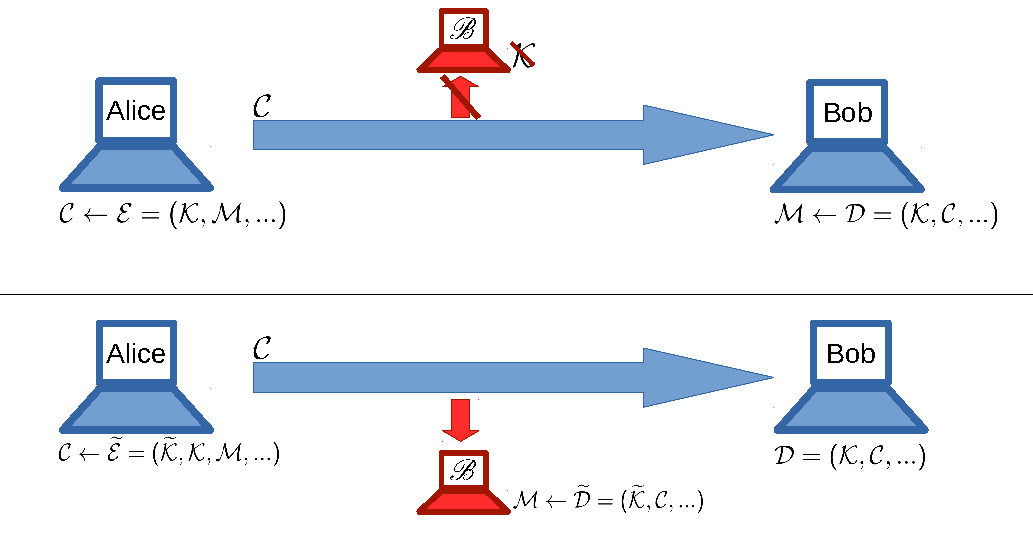
\includegraphics[width=\textwidth]{image/ideale_welt}
	\caption{Symmetrische Verschlüsselung in einer idealen Welt.}
	\label{fig:ideale_welt}
\end{figure}

\end{section}

\begin{section}{Korrektheit}
\label{sec:korrekt}

Letzteres ist essenzieller Bestandteil von Big Brothers Subversion. Jede Nachricht $M$ die von Alice verschlüsselt versendet wird muss mithilfe von $\mathcal{K}$ von Bob wieder zu $M$ entschlüsselt werden. Eben auch wenn Alice eine Subversion von $\Pi$ verwendet. Wir können sagen, dass ein Schema $\Pi = (\mathcal{K}, \mathcal{E}, \mathcal{D})$ korrekt ist, wenn der Empfänger den Chiffretext immer zu der gleichen ursprünglichen Nachricht $M$ entschlüsselt, die der Sender gesendet hat. Also wenn für alle Nachrichten gilt: $\mathcal{E}(\mathcal{K}, M_{1}) = \mathcal{C}_{1}$ und $\mathcal{D}(\mathcal{K}, \mathcal{C}_{2}) = M_{2}$, mit $\mathcal{C}_{1} = \mathcal{C}_{2}$ und $M_{1} = M_{2}$.

\end{section}

\begin{section}{Decryptability}
\label{sec:decryptability}

Eine weitere wichtige Eigenschaft beschreibt die Entschlüsselbarkeit einer Subversion $\widetilde{\Pi}$ relativ zu $\Pi$. Wenn $\widetilde{\Pi}$ ein korrektes Verschlüsselungs"-schema ist und die Funktion $\widetilde{\mathcal{E}}$ den Schlüssel $K$ und den Masterschlüssel $\widetilde{\mathcal{K}}$ verwendet, mit $K \neq \widetilde{\mathcal{K}}$, dann erfüllt $\widetilde{\Pi}$ die Eigenschaft Entschlüsselbarkeit. Allerdings nur jemand, der $\mathcal{K}$ hält, darf mit der Funktion $\mathcal{D}$ die Nachricht korrekt entschlüsseln. Wir gehen davon aus, dass $\mathscr{B}$ immer versucht diese Eigenschaft zu erreichen um nicht entdeckt zu werden.

\end{section}

\begin{section}{Detection Advantage}

Die Erfolgschancen von ASAs können an der Entdeckbarkeit gemessen werden. Eine Subversion ist von Alice oder Bob entdeckbar, wenn nicht gesagt werden kann, ob der Chiffretext $C$ von einer Subversion oder vom eigentlichen Schema $\Pi$ erzeugt wurde. Die Eigenschaft Entschlüsselbarkeit bildet hierfür die Basis. Wenn eine Entschlüsselung fehlschlägt, führt dies wahrscheinlich auch zum Entdecken der Subversion. Allerdings ist anzumerken, dass selbst wenn die Wahrscheinlichkeit Entdeckt zu werden hoch ist, beutet es nicht, dass ein Nutzer in der Lage ist eine Subversion zu entdecken.

\end{section}

\include{chapter/angriffe}

\chapter{Gegenmassnahmen}
\label{ch:Gegenmassnahmen}

An dieser Stelle ist es wichtig Schemen zu finden, die resistent gegen ASAs sind. Aus den Angriffen, die ich zuvor vorgestellt habe können wir lernen, dass wir Schemen nutzen sollten, die deterministisch und stateful sind. Vor allem stateless Schemen haben sich als gefährdet erwiesen, da Angriffe bei diesen besonders schwer zu entdecken sind. Wichtig hierbei ist, dass eigentliche Sicherheitseigenschaften wie Vertraulichkeit und Authentizität keinen Einfluss auf die Resistenz gegen ASAs bieten. Diese Resistenz wird nur in einer Klasse von symmetrischen Schemen sichergestellt, einer Klasse die von den Autoren unique ciphertext schemes genannt wird.

\begin{figure}[!ht]
	\centering
	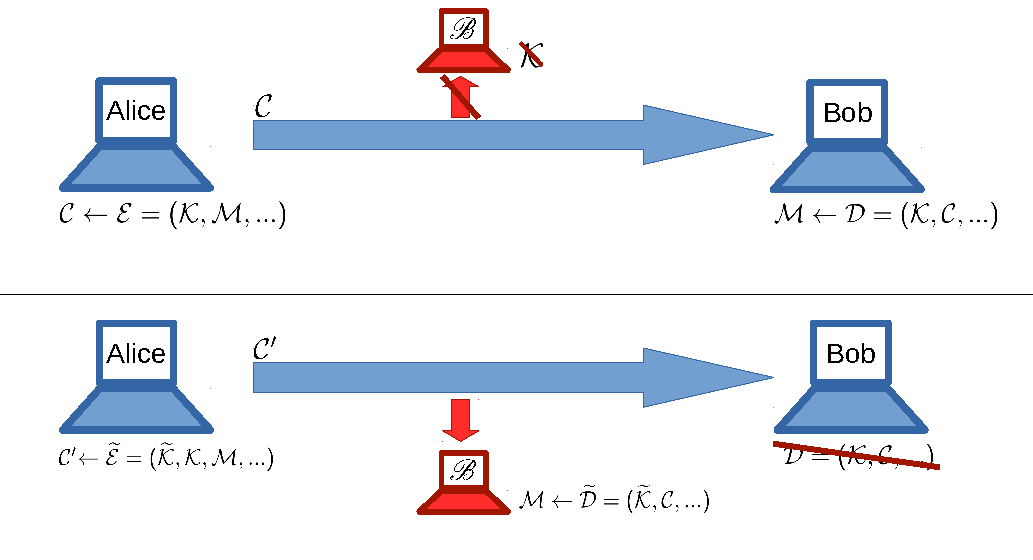
\includegraphics[width=\textwidth]{image/unique}
	\caption{unique chiphertext scheme.}
	\label{fig:unique}
\end{figure}

Um ein unique ciphertext Schema zu definieren, nehmen wir an, in dem symmetrischen Verschlüsselungsschema $\Pi = (\mathcal{K}, \mathcal{E}, \mathcal{D})$ soll folgendes gelten: Für jedes Tupel $(\mathcal{K}$, $\mathcal{M}, \mathcal{A}, \sigma$) gibt es höchstens ein $\mathcal{C}$, das entschlüsselt die Nachricht $\mathcal{M}$ unter $\mathcal{K}$ ergibt. Also wenn diese Abbildung injektiv ist (siehe \ref{fig:injektiv}), dann ist $\Pi$ ein unique ciphertext scheme.

\begin{figure}[!ht]
	\centering
	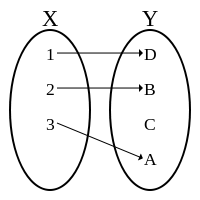
\includegraphics[width=0.3\textwidth]{image/Injection}
	\caption{Injektivität.}
	\label{fig:injektiv}
\end{figure}

Diese Eigenschaft trifft keineswegs auf alle Schemen zu. Für zwei verschiedene Chiffretexte $\mathcal{C} \neq \mathcal{C}^{'}$ muss also immer $\mathcal{D}(\mathcal{C}) \neq \mathcal{D}(\mathcal{C}^{'})$ gelten. Aus dieser Eigenschaft können wir Theorem \ref{theo:unique} erstellen. Wie in Abbildung \ref{fig:unique} zu sehen, sorgt eine Subversion von $\Pi$ dafür, dass ein Chiffretext $\mathcal{C}^{'} \neq \mathcal{C}$ beim Entschlüsseln bei Bob zu einer nicht korrekten Nachricht führt, also das Schema die Korrektheit aus Abschnitt \ref{sec:korrekt} nicht erfüllt. In diesem Fall würde die Subversion entdeckt werden.
	
\begin{theorem}
\label{theo:unique}

Sei $\Pi = (K, E, D)$ ein unique ciphertext scheme, dann gibt es kein Subversion $\widetilde{\Pi} = (\widetilde{K}, \widetilde{E}, \widetilde{D})$ von $\Pi$, mit der korrekt mit $\mathcal{D}$ entschlüsselt werden kann und $\mathscr{B}$ hat keine Erfolgschancen gegen $\Pi$.

\end{theorem}


\chapter{Zusammenfassung}
\label{ch:Zusammenfassung}


\nocite{BPR}
\pagenumbering{Roman}
\bibliography{bib/Literatur}
%\lstlistoflistings
\listoffigures

\end{document}